\documentclass{scrartcl}
\usepackage{amsmath,amssymb,commath,graphicx,enumerate,listings}
\setkomafont{disposition}{\normalfont\bfseries}

\title{Mat 354}
\subtitle{Homework 9}
\author{Kenny Roffo}
\date{Due October 26, 2015}

\begin{document}
\maketitle

All calculations were done in R.

\begin{enumerate}

\item \textbf{Poisson Process}\\

This is discussed at the end of the Poisson section in the text. The idea is pretty basic (although, of course, it can be elaborated on). If we agree that the number of contaminant particles in 1 cubic meter of air has a Poisson distribution with parameter / mean 2.4, then it follows that 2 cubic meters has a Poisson distribution with parameter 4.8. 1⁄2 cubic meter would be Poisson with parameter 1.2. And so on. (Technically this requires independence among different volumes of air.) The derivation of this is somewhat technical, but if you think about it in terms of approximating a Binomial, then it makes sense. If in 1 cubic meter you have 1000 trials with 0.0024 probability, then in 2 cubic meters you have a corresponding 2000 trials with the same probability. In general, if $\lambda$ is the base expected value of the count per 1 unit of “whatever”, and the distribution is Poisson, then the count per $a$ units is Poisson with parameter $\lambda^* = a\lambda$. The number of people to enter a bank in one minute in the afternoon is a Poisson random variable with mean 3.5. Use the Poisson Process to determine the following.\\

\begin{enumerate}[a)]
\item Determine the probability that, in one minute,
  \begin{enumerate}[i.]
    \item between 2 and 5 people (inclusive) enter
    \item over 7 people enter
  \end{enumerate}

  i. For a poisson distribution, the probability function is $p(y) = \frac{e^{-\lambda}\lambda^y}{y!}$. We could calculate this by calculating $\sum_{y=2}^{5}p(y)$, but instead we will use R's ppois function to calculate the distribution function at 1 and 5, then subtract them, which gives us the same thing. Upon doing so we find the probability that between 2 and 5 people enter during the minute is 0.7217.\\
  
  ii. To calculate the probability that over 7 people enter during one minute in the afternoon, we will simply subtract from 1 the probability that 7 or less people enter during that minute. We do so by calculating 1 $-$ ppois(7,3.5). This comes out to be 0.0267.\\

\item What is the distribution of the number of people who enter in a 5 minute period?

  This distribution is a poisson with $\lambda^* = 5\lambda = 17.5$\\

\item For a five minute period, determine the probability that
  \begin{enumerate}[i.]
    \item between 10 and 25 people (inclusive) enter
    \item over 35 people enter
  \end{enumerate}

We solve these two problems in the same manner from part a, but with the new poisson distribution.

  i. ppois(25,17.5) $-$ ppois(9,17.5) $=0.9460$
  
  ii. 1 $-$ ppois(35,17.5) $=0.00007059$\\

\item For a ten minute period, determine the probability that
  \begin{enumerate}[i.]
    \item between 20 and 50 people (inclusive) enter
    \item over 70 people enter
  \end{enumerate}
  Now we have $\lambda^* = 35$. Same calculations:

  i. ppois(50,35) $-$ ppois(19,35) $=0.9911$
  
  ii. 1 $-$ ppois(70,35) $=0.00000006068$\\

\item Complete the table. Here the second and third columns are the probabilities that the rate of entry averages in the given way.

\begin{center}
\begin{tabular} { c|c|c }
minutes&between 2 and 5 people per minute&over 7 people per minute\\
\hline
1&&\\
5&&\\
10&&\\
\end{tabular}
\end{center}

These are alternate ways of stating the above problems.

\begin{center}
\begin{tabular} { c|c|c }
minutes&between 2 and 5 people per minute&over 7 people per minute\\
\hline
1&0.7217&0.0267\\
5&0.9460&0.00007059\\
10&0.9911&0.00000006068\\
\end{tabular}
\end{center}

\item In general, then, the number of entrants into the bank in a period of a minutes has a Poisson distribution with parameter $3.5a$. Write an expression for the probability that at least one person enters the bank in a period of $a$ minutes. What happens to this probability as $a\rightarrow\infty$? Argue your answer with an appropriate limit calculation.

Now we have $\lambda = 3.5a$. The probability that at least 1 person enters the bank is, of course, 1 minus the probability that 0 people entered the bank. We see
$$p(0) = \frac{e^{-3.5a}(3.5a)^0}{0!} = e^{-3.5a}$$
Thus the probability that at least 1 person enters the bank in $a$ minutes is given by:
$$p(Y \ge 1) = 1 - e^{-3.5a}$$
It seems obvious that as $a$ goes to infinity, this probability goes to 1, but let's do a limit check:
\begin{align*}
  \lim_{a\rightarrow\infty}1 - e^{-3.5a} &= \lim_{a\rightarrow\infty}\left(1\right) - \lim_{a\rightarrow\infty}\left(e^{-3.5a}\right)\\
  &= 1 - \lim_{x\rightarrow\infty}\left(e^{-x}\right)\\
  &= 1 - 0\\
  &= 1
\end{align*}
So our limit check is good.
\end{enumerate}

\item \textbf{Help Me Find My Missing Data!}\\

A sample of $n$ (independent) observations was obtained from a Poisson distribution with parameter $\lambda$. I tabulated the data, but somewhere along the line I lost part of my table – I have no recollection of the number of times 0 occurred.\\

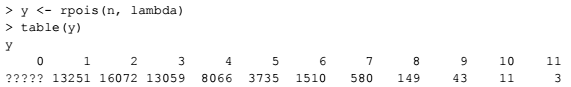
\includegraphics[keepaspectratio=true, scale=0.75]{2.png}

I’m looking for values for each of $n$ and $\lambda$. How many 0s were there? What I’m really after is a method that generally works to solve this problem (with instructions so that I can implement your method the next time I lose my 0s).

Note: This is all related to the “Zero-Truncated Poisson Distribution” which (of course) has applications “in real life.” A little research into that might lead into a systematic method that yields results that have true statistical validity (for which error margins can be computed and affixed).\\

Consider the following: $$p(1) = \frac{\lambda}{e^\lambda} \approx \frac{13251}{n}$$ and $$p(2) = \frac{\lambda^2}{e^\lambda2} = \frac{\lambda}{2}\frac{\lambda}{e^\lambda} \approx \frac{16072}{n}$$ Since the sample size is large, these approximations are likely to be pretty close. Notice what this implies:
\begin{align*}
  p(2) = &\frac{\lambda}{2}p(1) = \frac{16072}{n}\\
  \implies &\frac{\lambda}{2}\frac{13251}{n} = \frac{16072}{n}\\
  \implies &\lambda = \frac{2\cdot16072}{13251} \approx 2.43
\end{align*}
Thus $\lambda$ is about 2.43. Now we can plug that in to $p(2)$ to find $n$, and thus the number of 0s:
\begin{align*}
  &\frac{16072}{n} = \frac{\lambda^2}{e^\lambda2}\\
  \implies n &= \frac{2\cdot16072e^{\lambda}}{\lambda^2}\\
  &   = \frac{2\cdot16072e^{2.43}}{2.43^2}\\
  &   = 61833
\end{align*}
And now subtracting the sum of the numbers of 1-11 from 61833, we get the approximate number of 0s, which is 5354.

\end{enumerate}
\end{document}

